% The main file for TUM reports

\documentclass[12pt,a4paper,oneside,listof=totoc,bibliography=totoc,index=totoc,headsepline,footsepline,footinclude=false,BCOR12mm,DIV13]{scrbook}

% Set here the title, authors and other stuff to be used for the cover

\def\doctype{Bachelorarbeit in Informatik}
\def\title{On the new threats of social engineering exploiting social networks}
\def\titleGer{Neue Bedrohungen bei Sozialen Netzwerken im Bezug auf Social Engineering}
\def\author{Daniel Siegel}
\def\date{August 15, 2009}

% text to appear in the footer
\def\footertext{}

\usepackage{scrpage2}
\pagestyle{scrheadings}
\ifoot[\footertext]{\footertext} % \footertext set in INFO.TEX

\usepackage[utf8]{inputenc}
\usepackage[T1]{fontenc}
\usepackage[ngerman,english]{babel}
\selectlanguage{english}

\usepackage[pdftex]{graphicx}
\graphicspath{{figures/}}

\usepackage{cmbright}

\usepackage{ifthen}
\usepackage{subfigure}
\usepackage{colortbl}
\usepackage{multirow}
\usepackage{url}
\usepackage{color}
\usepackage{makeidx}
\usepackage{float}
\usepackage{rotating}

\usepackage{styles/tumlogo}
\usepackage{styles/shortoverview}
\usepackage{styles/secnum}


\usepackage[pdftex,colorlinks=true,linkcolor=red,citecolor=red,%
anchorcolor=red,urlcolor=red,bookmarks=true,%
bookmarksopen=true,bookmarksopenlevel=0,plainpages=false%
bookmarksnumbered=true,hyperindex=false,pdfstartview=%
]{hyperref}

\hypersetup{%
  pdftitle    = \title,
  pdfsubject  = {Bachelor thesis},
  pdfauthor   = {Daniel Siegel},
  colorlinks  = true,
  linkcolor   = blue,
  urlcolor    = red,
  breaklinks  = true,
}


%% Fancy chapters

% set the bibliography style
\bibliographystyle{styles/bauermaNum}
%\bibliographystyle{alpha}
%\bibliographystyle{plain}

% Disable single lines at the start of a paragraph (Schusterjungen)
% Disable single lines at the end of a paragraph (Hurenkinder)
\clubpenalty = 10000
\widowpenalty = 10000
\displaywidowpenalty = 10000

%% mark text as preliminary
\usepackage[draft,german,scrtime]{prelim2e}

% Commands to be used within the TUM report document

% comment that appears on the border - very practical !!!
\newcommand{\comment}[1]{\marginpar{\raggedright \noindent \footnotesize {\sl #1} }}

% page clearing
\newcommand{\clearemptydoublepage}{%
  \ifthenelse{\boolean{@twoside}}{\newpage{\pagestyle{empty}\cleardoublepage}}%
  {\clearpage}}



%\makeindex
%% inter line spacing
%\linespread{1.0}

\makeglossary

\begin{document}

  \frontmatter

  % The front cover for the TUM report document.

% correct BCOR - undo at the end !!!
\def\bcorcor{0.15cm}
\addtolength{\hoffset}{\bcorcor}

\thispagestyle{empty}

 \vspace{4cm}
\begin{center}
  \oTUM{4cm}

  \vspace{5mm}     
  \huge FAKULT{\"A}T F{\"U}R INFORMATIK\\ 
  \vspace{0.5cm}
  \large DER TECHNISCHEN UNIVERSIT{\"A}T M{\"U}NCHEN\\
  \vspace{1mm}

\end{center}

\vspace{15mm}
\begin{center}

  {\Large \doctype}
  \vspace{20mm}

  {\huge\bf \title}\\%[3ex]
  \vspace{15mm}

  {\LARGE  \author}
  \vspace{10mm}

  \begin{figure}[h!]
  \centering
   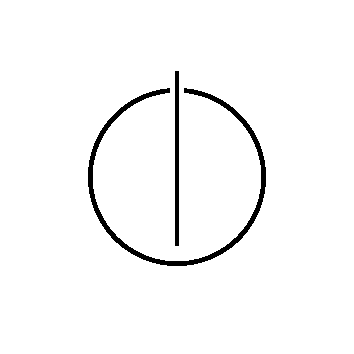
\includegraphics[width=4cm]{styles/informat.png}
  \end{figure}

\end{center}


  \clearemptydoublepage

  % The titlepage for the CAMP report document.

%--------------------------------------------------
% The title page
%--------------------------------------------------

\thispagestyle{empty}

\vspace{10mm}

\begin{center}
  \oTUM{4cm}

  \vspace{5mm}
  \huge FAKULTÄT FÜR INFORMATIK\\
  \vspace{0.5cm}
  \large DER TECHNISCHEN UNIVERSITÄT MÜNCHEN\\
  \vspace{1mm}
\end{center}

\vspace{10mm}
\begin{center}
  {\Large \doctype}
  \vspace{10mm}

  {\LARGE \textbf \title}\\
  \vspace{10mm}

  {\LARGE \textbf \titleGer}\\
  \vspace{10mm}

  \begin{tabular}{ll}
    \Large Author:     & \Large \author \\[2mm]
    \Large Supervisor: & \Large Univ.-Prof. Dr. Claudia Eckert \\[2mm]
    \Large Advisor:    & \Large Dipl.Inf. Werner Streitberger\\[2mm]
    \Large Date:       & \Large August 15, 2009
  \end{tabular}

  \vspace{5mm}

  \begin{figure}[h!]
  \centering
  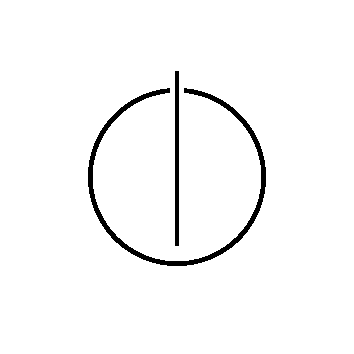
\includegraphics[width=4cm]{styles/informat.png}
  \end{figure}
\end{center}


  \clearemptydoublepage

\thispagestyle{empty}
\selectlanguage{ngerman}
  \vspace*{0.8\textheight}
  \noindent
  Ich versichere, dass ich diese Bachelorarbeit selbstständig verfasst und nur\\
  die angegebenen Quellen und Hilfsmittel verwendet habe.

  \vspace{15mm}
  \noindent
  M{\"u}nchen, den \today \hspace{5cm} \author
\selectlanguage{english}
\newpage


  \clearemptydoublepage
\phantomsection
\addcontentsline{toc}{chapter}{Acknowledgements}	

\vspace*{2cm}

\begin{center}
{\Large \bf Acknowledgments}
\end{center}

\vspace{1cm}

If someone contributed to the thesis... might be good to thank them here.


  % Abstract for the TUM report document
% Included by MAIN.TEX


\clearemptydoublepage
\phantomsection
\addcontentsline{toc}{chapter}{Abstract}	





\vspace*{2cm}
\begin{center}
{\Large \bf Abstract}
\end{center}
\vspace{1cm}

An abstracts abstracts the thesis!

  \tableofcontents

  \mainmatter

  \label{part:introAndBackgroundTheory}
  \chapter{Introduction}
\label{chapter:introduction}

\section{Problem and Motivation}

Social Networks, such as Facebook\footnote{\url{http://www.facebook.com}},
MySpace\footnote{\url{http://www.myspace.com}} or
Twitter\footnote{\url{http://www.twitter.com}} gained million of members on
their platforms in the last years. They are widely used in both private and
business networking. Services, like the one just mentioned, allow individuals
to present their own identity and to share and keep relationships to other
members of those services. Often, they are also presenting their information to
an unknown number of strangers.

This brings us not only to the question how useful a social network is for a
single user, but also if there are any drawbacks or risks.  Users often put
much and frequently sensitive data into their profiles, as for example
\cite{brown2008} shows.  This data however is stored centrally at the company
which provides the network and so the user looses the control over his
data~\cite{fraunhofer2008}.

There is of course a relation between the data the user entered and the user
himself. Following that thought, another person is not only able to extract the
data but also to obtain new information or rather interpretations, which were
not entered by the user.

Many studies, like \cite{fraunhofer2008,gross2005} show already, that this can
be a massive intervention into one's privacy. This work however wants to examine
whether such information are a security risk and can be used for attacks
against a company or an individual.

Of course, a distinction between employees of a certain company and private
users has to be made. For example, certain information can be harmless to an
individual, but very well a danger to a company \cite{mitnick2003}. In both
cases, however, a social engineer saves an additional step, for example a
telephone call or similar, to get that specific information. That step does not
only require extra work, but also the danger of being exposed. Without his
anonymity, a social engineer could not carry out an attack \cite{mitnick2003}.

Especially in big corporations spend hundreds of thousands or dollars for the
security of their IT-infrastructure. An attack at the IT-layer would therefore
often be very laborious. Therefore it is much simpler bypass the security
mechanisms through social engineering, as it very cheap and does not require
any superior technology \cite{winkler1995}. Commonly, a skilled social
engineering does not require anything more than a telephone for such attacks
\cite{mitnick2003}.

Concretely, this study wants to answer the following questioning:
How can data of individuals or companies automatically be extracted
from social networks and presented in a way, that it can be used for a social
engineering attack. In addition, countermeasures against automatic extraction
and social engineering attacks are going to be developed.

\section{Outline of the thesis}

\noindent {\textbf{Chapter 1}: Introduction}
\vspace{0.5em}\\
\noindent This chapter presents an overview of the thesis and it's purpose.
%Furthermore, it will discuss the threats and risks of social engineering and
%contain a glossary.

\noindent {\textbf{Chapter 2}: Related Work}
\vspace{0.5em}\\
\noindent The section will outline related works in the field of social
engineering, the attacks and countermeasures. It will present common attacks
and how companies and individuals can protect themselves against such attacks.

\noindent {\textbf{Chapter 3}: Analysis of the social network \Twitter}
\vspace{0.5em}\\
\noindent The study takes a deeper look at the social network \Twitter. It will
show the drawbacks and risks of such social networks, the data, which can be
extracted automatically, how sample attacks could look like and finally the
countermeasures against such attacks.

\noindent {\textbf{Chapter 4}: Design, analysis and implementation of a prototype}
\vspace{0.5em}\\
\noindent In this chapter, a prototype, who automatically can harvest data and
present it in a way, that it can be used for social engineering attacks, is
developed. The usual software engineering methods are used.

\noindent {\textbf{Chapter 5}: Evaluation}
\vspace{0.5em}\\
\noindent This chapter wants to examine, whether the already described attacks
can be achieved by using the prototype and therefore shows a sample attack. It
will analyse the attack and evaluate the risk against a company or an
individual.

\noindent {\textbf{Chapter 6}: Conclusion}
\vspace{0.5em}\\
\noindent The thesis finally concludes draws together the main findings of the
study.

\section{Glossary}

  \chapter{Related Work}
\label{chapter:relatedwork}


\section{Mögliche Social Engineering Angriffe}
\subsection{\glqq{}Digitale\grqq{} Angriffe}
\subsubsection{Phishing}
\subsubsection{Baiting}
\subsubsection{\dots}
\subsection{\glqq{}Analoge\grqq{} Angriffe}
\subsubsection{Pretexting}
\subsubsection{Identitätsdiebstahl}
\subsubsection{\dots}
\section{Schutzmöglichkeiten vor Social Engineering Angriffen bei
Privatpersonen und Unternehmen}
\subsection{Awareness}
\subsection{Unternehmens-Policy}
\subsection{Abschottung von Informationen}
\subsection{Schulung der Mitarbeiter}
\subsection{Technische Schutzmöglichkeiten}
\subsection{\dots}

  \chapter{Analyse des Sozialen Netzwerkes \glqq{}twitter\grqq{}}
\label{chapter:analyse}

\section{Begründung der Wahl dieses Sozialen Netzwerkes}
\section{Bedrohungen und Risiken}
\section{Relevante Daten und das Sicherheitsrisiko derselben bei Privatpersonen
und Unternehmen}
\subsection{Schwierigkeit relevante Daten zu extrahieren}
\subsection{Onthologie und Kategorisierung der Informationen}
\subsection{Automatisierte Extrahierung und Auswertung}
\section{Durchführung der Angriffe}
\section{Schutzmöglichkeiten}

  \chapter{Design, Analyse und Implementierung eines Prototypen}
\label{chapter:prototype}

\section{Zielsetzung}
\section{Beschreibung und Entwurf des Prototyps mit geeigneten Methoden des
Software Engineering}
\subsection{Use Cases}
\subsection{Sequence Diagramme}
\subsection{Klassendiagramme}
\subsection{\dots}
\section{Begründung gewählter Programmiersprachen, Tools und Bibliotheken}
\section{Dokumentation und Erklärung relevanter Stellen im Quellcode des
Prototyps}

  \chapter{Evaluation}
\label{chapter:evaluation}

\section{Demonstration eines Angriffes mithilfe des Prototyps}
\section{Prinzipielle Machbarkeit und Extrapolation auf andere Angriffe}

  \chapter{Zusammenfassung und Ausblick}
\label{chapter:zusammenfassung}



  \part*{Appendix}
  \addcontentsline{toc}{part}{Appendix}

  \appendix

  \chapter{Detailed Descriptions}
%\section{Detailed Validation Results}
\label{chapter:DetailedDescriptions}
Here come the details that are not supposed to be in the regular text.

  \clearemptydoublepage

  \bibliography{bibliography/literature}

\end{document}
